\section{Modelagem dos Agentes}
\label{sec:modelagem}

Como o eProfile é um modelo onde é necessário inferir informações de forma autônoma a respeito de dados armazenados em uma ontologia, a tecnologia de agentes autônomos foi escolhida para o desenvolvimento. A metodologia utilizada para a modelagem é a Prometheus \cite{prometheus}. Esta metodologia define um processo detalhado para a especificação, projeto, implementação e teste/depuração de sistemas de software orientados a agentes. \cite{prometheus-book}

\begin{figure}
  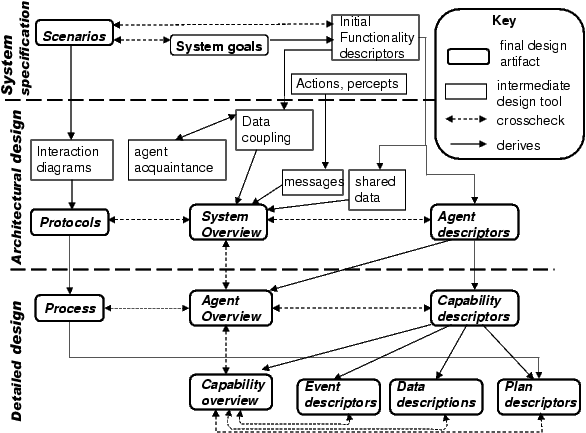
\includegraphics[width=0.8\textwidth]{imagens/prometheus.png}
  \caption[Metodologia Prometheus]{Processo de projeto segundo a metodologia Prometheus \cite{prometheus-book}}
  \label{fig:metodologia}
\end{figure}

A metodologia Prometheus, ilustrada na Figura~\ref{fig:metodologia} define que o primeiro passo da modelagem de um sistema é a identificação dos objetivos inciais do sistema. De acordo com o modelo do eProfile, os objetivos do sistema são:

\begin{itemize}
  \item Gerenciar múltiplos perfis;
  \item Comunicar-se com um (ou mais) gerenciadores de trilhas;
  \item Receber as regras de processamento dos clientes;
  \item Inferir dados de perfil através da análise das trilhas, de acordo com as regras definidas pelos clientes;
  \item Aceitar requisições de informações de perfil pelos clientes.
\end{itemize}

O modelo do eProfile é composto por três agentes: (i) conversor, (ii) regulador e (iii) raciocinador.

\todo[inline]{Mostrar a modelagem dos agentes, de acordo com a metodologia Prometheus}

%%%%%%%%%%%%%%%%%%%%%%%%%%%%%%%%%%%%%%%%%%%%%%%%%%%%

\subsection{Conversor}
\label{sec:conversor}

O \textbf{agente conversor} é responsável por realizar a conversão dos dados da trilha do gerenciador de trilhas (externo) para a ontologia de trilha do eProfile (interno). A trilha do gerenciador pode ser disponibilizada em qualquer formato e por qualquer meio, desde que o eProfile ofereça suporte ao gerenciador de trilhas específico. O agente conversor tem também a responsabilidade de verificar, a cada período pré-determinado, atualizações nos dados disponibilizados no gerenciador.

%%%%%%%%%%%%%%%%%%%%%%%%%%%%%%%%%%%%%%%%%%%%%%%%%%%%

\subsection{Regulador}
\label{sec:regulador}

O \textbf{agente regulador} realiza o recebimento das regras enviadas pela aplicação. Uma vez que as regras sejam recebidas, elas são validadas e, se forem consideradas válidas, são armazenadas na base de regras. A aplicação é então informada do aceite ou rejeição. O agente pode rejeitar uma regra se: (i) a regra for inválida ou (ii) se for verificado que a execução da regra irá consumir recursos excessivos do servidor.

%%%%%%%%%%%%%%%%%%%%%%%%%%%%%%%%%%%%%%%%%%%%%%%%%%%%

\subsection{Raciocinador}
\label{sec:raciocinador}

O \textbf{agente raciocinador} é responsável pela inferência das trilhas de acordo com as regras enviadas pela aplicação, e posterior atualização do perfil da entidade. A execução do agente não necessita que o cliente ou o gerenciador de trilhas esteja conectado, e ocorre da seguinte forma:

\begin{enumerate}

\item O agente verifica as regras, comparando a data da útlima execução da regra com a freqüência de execução, definida pela aplicação na criação da regra.

\item Caso seja o momento da execução da regra, a mesma é executada através da biblioteca externa HermiT \cite{motik09}.

\item Caso a regra tenha sido executada com sucesso, o resultado da regra é atualizado no perfil. Em caso de insucesso, o erro é enviado para a aplicação no momento que a mesma se reconectar.

\end{enumerate}
